\section{Integrationstest}
Under integrationen af de samlede moduler opstod der flere problemer, som blev løst gennem forskellige fejlsøgninger af det samlede system. Herunder vil de brugte testmetoder under integrationen blive forklaret.\\

For at kunne se hvordan enhederne i systemet kommunikerer, er der på de forskellige softwareenheder lavet funktioner, der kan ''sladre'' gennem UART-kommunikation. Dette sammen med programmet Tera Term(terminal) giver mulighed for at se præcis hvor i koden de individuelle enheder er. Et kode eksempel på dette kan ses på Figur \ref{fig:sladrehank}.\\

\begin{figure}[h]
	\begin{lstlisting}
...
	if (debugging)
	{
		getMyTxUART()->sendString("Checking time, current time is: ");
		getMyTxUART()->sendNumber(minutes);
		getMyTxUART()->sendChar(':');
		getMyTxUART()->sendNumber(seconds);
		getMyTxUART()->sendString("\n\r");
	}
...
	\end{lstlisting}
	\caption{Eksempel på en sladrehank fra Transmitter Time klassen}
	\label{fig:sladrehank}
\end{figure}

Det kan ske at koden fortæller, at den gør en ting, men i realiteten sker dette ikke. For at kunne analysere sådan et problem, er det ofte lettere at analysere direkte på rådata via kommunikationen. Her er oscilloskop'et et stærkt fejlsøgningsredskab, da det er muligt at se, hvad der sker direkte på kommunikationsvejen mellem de individuelle moduler. Ved analysering af spændingen på indgange og udgange af systemets individuelle enheder kan en fejl hurtigt indrammes om det er et hardware eller software problem. Et eksempel på rådata, der kan analyseres, kan ses på Figur \ref{fig:oscilloskop}.\\

\begin{figure}[h]
	\centering
	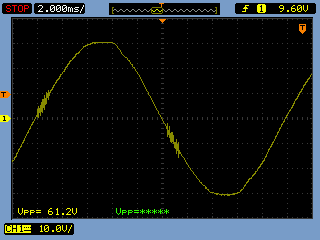
\includegraphics[scale=0.75, trim=0 0 0 0, clip=true]{Projektbeskrivelse/Integrationstest/billeder/Oscilloskop.png}
	\caption{Oscilloskop screenshot af X.10 på $18V AC$}
	\label{fig:oscilloskop}
\end{figure}

Med standard frekvens på $50Hz$ kan det være svært at analysere på systemet, da der sker to nulgennemgange for hver periode der kører. Dermed kan systemet kommunikere med $100$ bits i sekundet. For at komme uden om dette problem er der blevet testet med en lavere frekvens, helt ned til $1Hz$, under systemets integration. Dette gør det muligt at aflæse data på LED'er på STK500 kittene.